\documentclass[sigplan,review,anonymous]{acmart}
\setcopyright{none}
%
\usepackage{tikz}
\usepackage{amssymb}
\usepackage{algorithm}
%
\usepackage{graphicx}
% Used for displaying a sample figure. If possible, figure files should
% be included in EPS format.
%
% If you use the hyperref package, please uncomment the following line
% to display URLs in blue roman font according to Springer's eBook style:
% \renewcommand\UrlFont{\color{blue}\rmfamily}
\AtBeginDocument{%
  \providecommand\BibTeX{{%
    \normalfont B\kern-0.5em{\scshape i\kern-0.25em b}\kern-0.8em\TeX}}}

\begin{document}
\settopmatter{printacmref=false}
\title{Online Verification of Commutativity}
%
%\titlerunning{Abbreviated paper title}
% If the paper title is too long for the running head, you can set
% an abbreviated paper title here
%
\author{First Author}
\email{email}
\author{Second Author}
\authornotemark[1]
\email{email 2}
\affiliation{%
  \institution{Cornell University}
  \streetaddress{address}
  \city{Ithaca}
  \state{New York}
  \postcode{14850}
}

\author{Third Author}
\email{email 3}

\begin{abstract}
Commutative diagrams arise in many systems, such as an implicit type conversion graph in some programming languages.
It can be useful in program analysis to verify that a diagram representing conversions remains commutative over the course of its construction.
A naive approach to solving the problem would take factorial time, and the presence of cycles could potentially lead to an infinite number of paths to check. Previous work provides an algorithm for the special case of acyclic diagrams that verifies that a given diagram commutes in $O(|V|^4|E|^2)$ time, where V is the set of vertices in the diagram, and E, the set of edges. 
We present an algorithm that given a diagram and an edge to add to it, verifies that the resultant diagram commutes in $O(|V|(|E| + |V|)$ time. For the case when checking the equality of paths is expensive, we present an optimization that runs in $O(V^4)$ time but reduces to the minimum possible number of equality checks. We evaluate the algorithms against baselines, and see its practical application in the compiler of a domain specific language for geometry types. As a demonstration of the more general applicability of the algorithm, we use it to identify discrepancies in a  currency conversion graph.
\end{abstract}
%
%
%

\maketitle

\section{Introduction}
Many systems can be understood as a category, with a collection of sets, and some transformation functions between the sets- for example, in programming languages, type systems with coercion. If a directed graph is constructed with the sets as nodes and functions as edges between the nodes, then by construction, in the new graph, choice of path should not matter- any choice of path should yield the same transformation between any two nodes. Each object has a unique representation in a given set in the system, so the transformation mapping between any two nodes should not depend on choice of path used to obtain the transformation. We will use the term "diagram" to refer to such graphs with their associated sets (vertices) and transformations (edges).

Since such commutative diagrams arise in many systems, it is often useful to be able to perform verification and ensure the graphs in question are indeed path independent. 
We formalize the problem as checking the commutativity of a diagram incrementally.
A diagram is said to commute when on selecting any two vertices, any directed path leads to the same result by composition.
Naively checking if all paths in a given graph are path independent could require a number of function equality checks as bad as factorial in the number of nodes, since a path consists of an ordering of nodes. Further, the presence of cycles implies a potentially infinite number of paths. Previous work ~\cite{commutative} has identified an $O(|E|^2|V|^4)$ algorithm to verify that an acyclic diagram commutes.

We present a polynomial time $O(|V|(|E|+|V|)$ algorithm to verify that commutativity of a graph is maintained over the course of online addition, assuming an oracle to check the abstract notion of equality of functions. The number of calls to the equality checking oracle required by the algorithm is asymptotically tight. With an additional $O(|V|^4)$ optimization step, is is possible to use instead the minimal possible number of equality checks, should these checks be expensive. We compare our solution to three baselines: a naive checking of all path pairs, with only special handling for cycles, a check for all path pairs that involve the new edge, and with an algorithm suggested by previous work to solve the batch version of the problem for acyclic diagrams.

To evaluate our results we use two case studies.
First, in the domain specific geometry type language \textit{Gator}, our algorithm is used to ensure that user defined transformations between spaces stay consistent, and the compiler, deterministic as it makes automatic conversion choices. As a second case study, the the algorithm is used to identify inefficiencies in a currency conversion graph.

\section{Formal Problem Setup and Terminology}

First, we formalize the notion of a diagram, drawing inspiration from Murota ~\cite{commutative}.

% A lot of this exposition is from the cited paper, I feel like I need to make this clearer to give proper credit, but not sure how.

We start with a directed graph G=(V,E) with sets attached to vertices and maps, to arcs. Each edge (u, v) in E corresponds to a function that maps elements of u to elements in v.
All the functions form a semigroup F, with multiplication denoted by $\circ$.
A semigroup is an algebraic structure with a set and an associative binary operation. We use it to represent functions in order to capture the one allowed operation- function composition.

The correspondence between edges and functions is stored as a mapping f:$E\rightarrow F$. f maps each edge to the function it represents.

A path is a sequence of edges. The edge-to-function mapping f can be naturally extended to paths. If path p=$e_1\circ e_2 ... e_n$ then $f(p)=f(e_1) \circ f(e_2) ... f(e_n)$.

Let $P_{all}$ is the set of all paths in G.

The notation $\partial^{+}(p)$ is used to indicate the start node of path p, and similarly $\partial^-(p)$ is the end node of path p. $\partial(p)$ maps to the tuple (start node of p, end node of p).

A pair of paths p and q is called \textit{parallel} iff their terminal nodes are the same, i.e., $\partial(p)=\partial(q)$.
The problem of checking if diagrams commute amounts to checking if the two members of every parallel pair that can be constructed is equal.

Let $R_{all}$ be the set of all parallel pairs of paths in the diagram.

The diagram commutes iff f(p)=f(q) $\forall (p,q)\in R_{all}$, which is to say, the compositions of the maps along any path connecting u to v is independent of choice of path. Here, equality of functions is defined by an equality oracle whose exact specifics will vary with the nature of the functions and the domain to which the diagram belongs.

\section{Baselines}

\subsection{Naive all-path check}
The naive solution is to verify that in every parallel pair in the diagram, the two paths are equal. However since cycles potentially introduce an infinite number of pairs, they must be dealt with separately.

Two situation can be imagined- the first, where the existence of the identity function from every node to itself is assumed as would describe most real world situations, and the second, where no such identity needs to exist.

When the identity is assumed, every cycle forms a parallel pair with an identity function on the terminal node. Therefore, the cycle must be verified to be equal to the identity on every node in the cycle. If this check succeeds for every elementary cycle in the diagram, then paths with multiple instance of the cycle must be equal to the version of the path without the cycle. It is therefore then enough to perform verification for all pairs where none of the path involves cycles. This is a finite set, bounded by $^{|E|!}C_2$. All elementary cycles in a diagram can be found in $O((|V|+|E|)(C+1))$ using Johnson's algorithm where C is the number of cycles, that can be greater than $2^{|V|}$. Thus the baseline is a factorial time algorithm that is nevertheless guaranteed to terminate.

Without the identity assumed, a cycle c forms a parallel pair with itself repeated twice- the pair (c, c;c). This verification needs to be performed for all elementary cycles. Further, if there is any "exit" or "entrance" into an elementary cycle- an edge that is not a part of the cycle whose one end is a node that belongs to the cycle- then it must be verified that the transformation represented by the edge is equal to the transformation represented by the edge and cycle composed (the cycle is pre-pended in the case of an edge directed away from the cycle and appended in the case of an edge directed into the cycle). Should this verification succeed, by logic similar to the previous case, it must be that all paths (including complex cycles) that include the elementary cycle must be equal to version of the paths without the cycle (since a segment of the path with the cycle has already been verified to be equal to a version of that segment without the cycle). Once again this is a factorial time, terminating algorithm.

\subsection{Naive algorithm for online addition}

Since we solve the question of online addition, where the original diagram is path independent and a new edge is added, the naive baseline can be improved to verify only parallel pairs that have been affected by the addition of the new edge. Pairs that do not involve the new edge must continue to be path independent because they already belonged to the old diagram.

The cycle checking steps can also be improved upon. In the case where the identity is assumed, only elementary cycles passing through the new edge need to be verified to be equal to the identity. When the identity is not assumed, cycles that include one of the nodes of the new edge must be checked for the new exit or entry point that the new edge becomes (if the cycle includes the source of the new edge then the cycle followed by the new edge must be equal to the new edge alone and if the cycle include the sink then the new edge followed by the cycle must be equal to the new edge).
Additionally, all cycles that include the new edge would need full verification like in the batch algorithm- the cycle would have to be equal to itself composed with itself, and would have to be verified for all its entry and exit points.

Now, the commutativity of the original diagram could be used to narrow down the set of pairs to verify. Pairs where both paths do not involve the new edge would remain equal, but also, pairs where both paths involved the new edge would have to be equal. To see why this is true, each path could be thought of as consisting of the composition of three segments, the first segment from the common source to the source of the new edge, the second, the new edge itself, and the third, from the sink of the new edge to the common sink of the parallel pair. The first segment of both pairs would have to be equal because they existed in as parallel pairs in the original diagram, and similarly the third segments would also have to be equal. The second segments, consisting of the same edge, would also have to be equal. Therefore the composition of these three equal components would be equal. Note that the new edge could only appear once because cycles have already been dealt with and none of the paths under consideration hit a node twice. Thus we are left only to verify the pairs where exactly one of the paths includes the new edge.

a "two-flip tolerant" path search could be used to identify the pairs of paths where exactly one path includes the new edge. 

\subsubsection{Two flip tolerant path search}
In a normal directed graph path, only forward edges, i.e. edges that go outward from the current node, are considered. 
On the other hand, the \textit{two flip path} goes through up to three phases: in the first phase, only backward edges- pointing inward to the current node- are accepted. In the second phase, only forward edges are accepted, and in the third phase, again only backward edges are accepted. As a consequence, there is a node in the path for which both path edges are oriented outwards, that lies between the first and second phase. This will be referred to as the \textit{first flipping point}. Similarly, there is a \textit{second flipping point} between the second and third phase, for which both path edges point inwards.

Consider the situation where a new edge from source node S to sink T is being added to a diagram.
A two flip tolerant path from S to T would correspond to a new pair of parallel paths- flipping point 1 would be the source of both paths, and flipping point 2, the sink. The first path would correspond to the second phase of the flip tolerant path search, and the second path, involving the new edge, would correspond to composing the first phase of the two flip path, the new edge, and the third phase.

To present this idea diagrammatically, we represent path phases with arrows (note that these are the composition of many edges, not a single edge). The new edge is represented with a dashed arrow.

\begin{center}
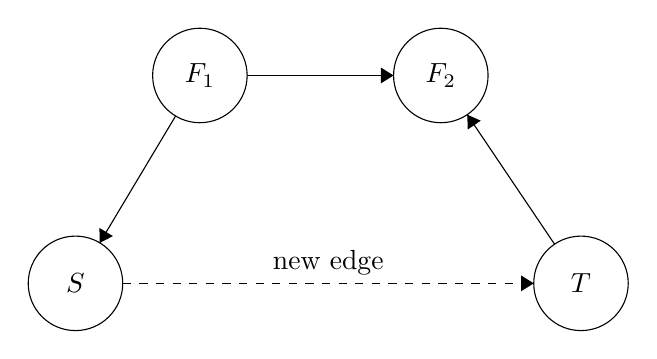
\begin{tikzpicture}[scale=0.2]
\tikzstyle{every node}+=[inner sep=0pt]
\draw [black] (18.1,-36.1) circle (3);
\draw (18.1,-36.1) node {$S$};
\draw [black] (50.2,-36.1) circle (3);
\draw (50.2,-36.1) node {$T$};
\draw [black] (26,-22.9) circle (3);
\draw (26,-22.9) node {$F_1$};
\draw [black] (41.3,-22.9) circle (3);
\draw (41.3,-22.9) node {$F_2$};
\draw [dashed] (21.1,-36.1) -- (47.2,-36.1);
\fill [black] (47.2,-36.1) -- (46.4,-35.6) -- (46.4,-36.6);
\draw (34.15,-35.6) node [above] {new edge};
\draw [black] (24.46,-25.47) -- (19.64,-33.53);
\fill [black] (19.64,-33.53) -- (20.48,-33.1) -- (19.62,-32.58);
\draw [black] (29,-22.9) -- (38.3,-22.9);
\fill [black] (38.3,-22.9) -- (37.5,-22.4) -- (37.5,-23.4);
\draw [black] (48.52,-33.61) -- (42.98,-25.39);
\fill [black] (42.98,-25.39) -- (43.01,-26.33) -- (43.84,-25.77);
\end{tikzpicture}
\end{center}
Here, (S, $F_1$, $F_2$, T) is a two flip tolerant path. ($F_1$, S, T, $F_2$) is a new path, created because of the addition of (S,T), that conflicts with ($F_1$, $F_2$).

The two flip tolerant path search returns the set of all paths between a given source and sink that have up to two flips (paths that omit one or more of the three phases are also accepted).

The \textit{path extraction algorithm} then transforms the output of the two flip path search to the set of new pairs of parallel paths that arise in the diagram due to its addition, that need to be verified.

\paragraph{Path extraction algorithm}
The purpose of this algorithm is to derive the conflicting pairs that a given two-flip tolerant path corresponds to.

Let the new edge added to the diagram be (S, T).
It has already been shown how each path corresponds to a conflicting pair in the case where a path has two flips. When a path has only the first flip (which is to say, the third phase of the path is missing), but not the second flip, sink node T can be treated as the sink of the two conflicting path, while the first flipping point remains the source. Similarly when only the second flipping point is present then it is the sink, and S is the source. Finally when no flipping points are present, there are two possibilities. 
Either the path is oriented from S to T, in which case the conflicting paths are simply the edge (S, T) and the entire flip-less path, or the path is oriented from T to S. In this case, we have found a cycle that has already been dealt with.


\paragraph{Theorem} The result of the two-flip tolerant path search from the source to the sink node of an edge that is to be newly added, followed with the path extraction algorithm has a one-to-one correspondence to the set of new parallel pairs with exactly one path passing through the new edge, with neither paths containing any cycles.

\paragraph{Proof}

Every element in the output of the path extraction algorithm was by construction a conflicting pair.

It remains to show that every new conflicting pair corresponds to a two flip tolerant path. Let the common source be $F_1$ and common sink be $F_2$. 

Only one path passes through (S, T), which we will name path 1. We construct a two flip tolerant path from S to T: phase 1 is the segment of path 1 from $F_1$ to S, phase 2 is path 2, and phase 3 is the segment of path 1 from T to $F_2$. It is possible that some of $F_1, F_2, S$ and $T$ coincide, in which case the corresponding segments between them disappear, and the resultant path has fewer than two flips.

We have shown that all paths that need verification are caught by the two flip tolerant search followed with path extraction.

\paragraph{Implementation}
*Copy in python code from implementation? Appendix?*

This algorithm is also in the worst case as bad as factorial in the number of nodes. However, in the average case, it significantly outperforms the naive batch baseline. For sparse diagrams it is even competitive with our ultimate polynomial solution. Average case heuristic analysis will be presented in the evaluation section.

\subsection{Optimal solution for batch problem}
Murota's main result ~\cite{commutative} is a solution to the question of whether a given acyclic diagram commutes that returns the minimal number of equality checks. The paper describes the following algorithm to find the ($V^2E$ bounded) minimal set of pairs that needs to be checked.

A diagram's structure can result in some redundancy, in the sense that verifying a subset of pairs can imply the verification of path pairs that aren't in the subset.
For example, in the figure below, verifying $p_1$ and $p_2$ implies that the paths in $p_3$ are equal too.

\begin{center}
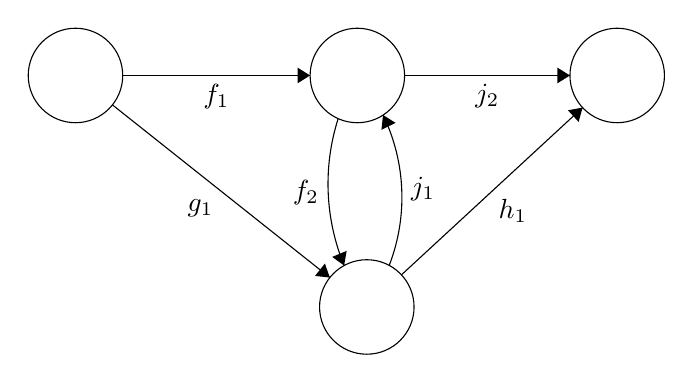
\begin{tikzpicture}[scale=0.2]
\tikzstyle{every node}+=[inner sep=0pt]
\draw [black] (12,-15.8) circle (3);
\draw [black] (30.5,-30.5) circle (3);
\draw [black] (46.4,-15.8) circle (3);
\draw [black] (29.9,-15.8) circle (3);
\draw [black] (15,-15.8) -- (26.9,-15.8);
\fill [black] (26.9,-15.8) -- (26.1,-15.3) -- (26.1,-16.3);
\draw (20.95,-16.3) node [below] {$f_1$};
\draw [black] (14.35,-17.67) -- (28.15,-28.63);
\fill [black] (28.15,-28.63) -- (27.84,-27.74) -- (27.21,-28.53);
\draw (19.94,-23.64) node [below] {$g_1$};
\draw [black] (29.063,-27.873) arc (-157.62406:-197.70132:13.638);
\fill [black] (29.06,-27.87) -- (29.22,-26.94) -- (28.3,-27.32);
\draw (27.49,-23.25) node [left] {$f_2$};
\draw [black] (31.53,-18.309) arc (25.84176:-21.16715:11.992);
\fill [black] (31.53,-18.31) -- (31.43,-19.25) -- (32.33,-18.81);
\draw (33.28,-23.03) node [right] {$j_1$};
\draw [black] (32.9,-15.8) -- (43.4,-15.8);
\fill [black] (43.4,-15.8) -- (42.6,-15.3) -- (42.6,-16.3);
\draw (38.15,-16.3) node [below] {$j_2$};
\draw [black] (32.7,-28.46) -- (44.2,-17.84);
\fill [black] (44.2,-17.84) -- (43.27,-18.01) -- (43.95,-18.75);
\draw (39.77,-23.64) node [below] {$h_1$};
\end{tikzpicture}

$p_1$=($f_1;f_2$, $g_1$)\\
$p_2$=($j_1;j_2$, $h_1$)\\
$p_3$=($f_1;h_1$, $f_1;j_2$)
\end{center}


The approach in the algorithm, at a high level, is to define a function that takes in a subset of pairs and returns the subset of pairs whose verification is implied by the verification of the input set. Then, greedy elimination of redundancies is performed until a minimal set is reached.

A bilinking is defined to be a parallel pair that is disjoint but for their terminal nodes. The set of all bilinkings is $R_0$.
In an acyclic diagram, if all bilinkings are equal, all parallel pairs must also be equal since they any given pair can be expressed as a composition of bilinkings.

Define $r_1>r_2$ for bilinkings $r_1$ = $\{p_l,q_l\}$, $r_2$= $\{p_2, q_2)$ $\in$ $R_0$, if there exists a path p such that $\partial p=\partial r_1$ and p contains $p_2$.
The $\langle\rangle$ function is defined as:
$\langle r \rangle = \{ s\in R_0| r>s\}$.

For bilinking s, let F(s) be the vector in $\mathbb{F}2^{|E|}$ representing the edges present in s (there is a dimension corresponding to each edge, the $n^{th}$ dimension of F(s) is 1 if the corresponding edge is in s, and 0 otherwise). Let this function be extended to sets, so that for some set of bilinkings S, F(S) = $\{ F(s) | s\in S \}$.

for a set of bilinkings r, the closure function cl is defined as:
cl(r) = $\{ s\in R_0|$ s is linearly dependent on $F(r) \}$.

The closure function on r basically captures all the pairs that can be made by made by composing or "gluing together" the bilinkings in r. 
The aforementioned $\langle\rangle$ function captures the orientation of paths, and can be used to constrain compositions to be in the right direction. 

Using these two function we finally define the function $\sigma$ on a set of bilinkings r as
$\sigma(r) = \{s \in R_0 | s\in cl(R\cap \langle s \rangle) \}$.
This is the function used to capture all the pairs whose verification is implied by the verification of pairs in r.

$\sigma$ is used to iteratively check if a given pair is redundant. bilinkings are eliminated until a minimum "spanning" subset is reached.

An implementation of the described algorithm is

\begin{verbatim}
Graph existingGraph;
R_s = {}
for each node v in V:
    # Let the subsection of the graph reachable from v be S.
    S = existingGraph.extractReachableSection(v)
    # Create a minimum spanning tree of S
    T = createMinimumSpanningTree(S)
    # Find the excluded edges
    excludedEdges = S.edges - T.edges
    # Use these edges to create bilinkings
    for each edge e in excludedEdges:
        firstPath = T.findPath(source: e.source, sink: e.sink)
        R_s.addElement(new Bilinking(firstPath, e)
return R_s
\end{verbatim}

\begin{verbatim}
Find a spanning set Rs, = [r_1, ... ,r_k].

R := Rs,
    for i:=l to K do
        if r_i in sigma(R - r_i) then R:=R - r_i;
return R.

sigma(inputSet S, codomain = Rs):
    output = {}
    for bilinking in Rs:
        smallerPairs = {}
        for candidateBilinking in Rs:
            if exists path(source: bilinking.source, sink:candidateBilinking.source) and
            exists path(source: candidateBilinking.sink, sink: bilinking.sink):
                smallerPairs.add(candidateBilinking)
        # Check if there's a linear dependence between the bilinking and smallerPairs
        # vectorize(pair) returns a vector with a dimension for each edge in the graph,
        # with a 1 if pair includes that edge and 0 if it doesn't.
        matrix = [vectorize(pair) for pair in smallerPair]
        matrix = matrix+[vectorize(bilinking)]
        # if there is a linear dependence
        if determinant(matrix)%2==0:
            output.add(bilinking)
    return output
                
\end{verbatim}

The proof of correctness can be found in Murota\cite{commutative}, 
The number of checks returned by the algorithm is at worst $O(|V|^2|E|)$. The overall run time of an optimized implementation is $O(|V|^4|E|^2)$.

\section{Solving the online addition problem}

The solution presented here assumes that there is an implicit identity function on every node, as would be the case in most applications. However, a modified version of the algorithm for diagrams without this assumption is presented in the appendix. The modification is similar in spirit to what was described in the description of the naive baselines.

Like with the online baseline, we do not concern ourselves with parallel pairs where neither or both paths pass through the new edge.
The key observation that allows us to improve on the online baseline is that for a given (source, sink) pair only a single parallel pair needs to be verified. This is an implication of Theorem \ref{reductionRule}, expanded on later.
Theorem \ref{verifyingSet} shows that should our selected set of pairs along with cycles passing through the new edge be verified commutative, the entire diagram must commute. The approach is to identify a parallel pair with exactly one path through the edge for each (source, sink) pair.


\begin{verbatim}
Graph existingGraph;
Edge newEdge;

Set parallelPairs = new Set();
for S in existingGraph.Nodes():
    for T in existingGraph.Nodes():
        try:
            Path pathWithNewEdge = 
                FindPath(
                    graph: existingGraph, 
                    sourceNode: S,
                    sinkNode: newEdge.Source()) +
                newEdge as Path +
                FindPath(
                    graph: existingGraph, 
                    sourceNode: newEdge.Sink(), 
                    sinkNode: T)
            if (S==T):
                // Cycles are a speacial case.
                pathInOldGraph = identity(S)
            else:
                Path pathInOldGraph = FindPath(
                    graph: existingGraph, 
                    sourceNode: S, 
                    sinkNode: T);
            parallelPairs.add((pathInOldGraph, pathWithNewEdge));
        catch (pathFindingFailed Exception):
            // No comparable pairs from node {S} to node {T} 
            // that need to be checked
            continue

output parallelPairs;
\end{verbatim}

The try block is executed at most $O(|V|^2)$ times, so that this is the bound on the number of pairs verified.

The bound is asymptotically tight. This can be seen in the case where the graph contains 2N nodes besides S and T. We consider N of the nodes to be in group 1, and the other N to be in group 2. Every node in group 1 has a forward node to every node in group 2, as well as to S. T has a forward edge to every node in group 2. In this diagram, on the addition of edge (S, T), $N^2$ paths need to be verified which is polynomial in 2N+2.

Also notice that if trying to optimize for path length (say, if composing functions is expensive) then "find any path" can be replaced with "find shortest path".

An efficient implementation of the algorithm can run in $O(|V|(|V|+|E|))$ time at a $O(|V|^3)$ space cost. In such an implementation, path finding from a given source node to all potential sink nodes would be done in a single $O(|V|+|E|)$ breadth first search and the results memoized in $O(|V|^2)$ space.

\subsection{Optimization Step}

In the case where equality checks are very expensive, we begin by finding the minimal set of (source, sink) pairs such that checking for these pairs logically implies having checked the full diagram.

We observe that there are some redundancies in the diagram.

Consider the following situation:

\begin{center}
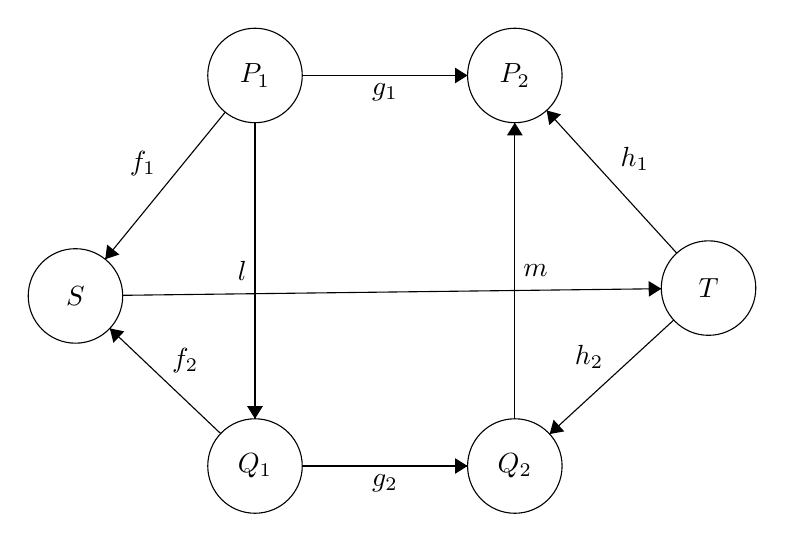
\begin{tikzpicture}[scale=0.2]
\tikzstyle{every node}+=[inner sep=0pt]
\draw [black] (16.6,-34.1) circle (3);
\draw (16.6,-34.1) node {$S$};
\draw [black] (56.8,-33.6) circle (3);
\draw (56.8,-33.6) node {$T$};
\draw [black] (28,-20.1) circle (3);
\draw (28,-20.1) node {$P_1$};
\draw [black] (44.5,-20.1) circle (3);
\draw (44.5,-20.1) node {$P_2$};
\draw [black] (28,-44.9) circle (3);
\draw (28,-44.9) node {$Q_1$};
\draw [black] (44.5,-44.9) circle (3);
\draw (44.5,-44.9) node {$Q_2$};
\draw [black] (31,-20.1) -- (41.5,-20.1);
\fill [black] (41.5,-20.1) -- (40.7,-19.6) -- (40.7,-20.6);
\draw (36.25,-20.6) node [below] {$g_1$};
\draw [black] (26.11,-22.43) -- (18.49,-31.77);
\fill [black] (18.49,-31.77) -- (19.39,-31.47) -- (18.61,-30.84);
\draw (21.74,-25.67) node [left] {$f_1$};
\draw [black] (25.82,-42.84) -- (18.78,-36.16);
\fill [black] (18.78,-36.16) -- (19.01,-37.08) -- (19.7,-36.35);
\draw (23.57,-39.02) node [above] {$f_2$};
\draw [black] (31,-44.9) -- (41.5,-44.9);
\fill [black] (41.5,-44.9) -- (40.7,-44.4) -- (40.7,-45.4);
\draw (36.25,-45.4) node [below] {$g_2$};
\draw [black] (54.59,-35.63) -- (46.71,-42.87);
\fill [black] (46.71,-42.87) -- (47.64,-42.7) -- (46.96,-41.96);
\draw (49.21,-38.76) node [above] {$h_2$};
\draw [black] (54.78,-31.38) -- (46.52,-22.32);
\fill [black] (46.52,-22.32) -- (46.69,-23.25) -- (47.43,-22.57);
\draw (51.19,-25.39) node [right] {$h_1$};
\draw [black] (28,-23.1) -- (28,-41.9);
\fill [black] (28,-41.9) -- (28.5,-41.1) -- (27.5,-41.1);
\draw (27.5,-32.5) node [left] {$l$};
\draw [black] (19.6,-34.06) -- (53.8,-33.64);
\fill [black] (53.8,-33.64) -- (52.99,-33.15) -- (53.01,-34.15);
\draw [black] (44.5,-41.9) -- (44.5,-23.1);
\fill [black] (44.5,-23.1) -- (44,-23.9) -- (45,-23.9);
\draw (45,-32.5) node [right] {$m$};
\end{tikzpicture}
Each arrow represents a path, and (S,T) is the new edge being added.
\end{center}
\begin{theorem}
\label{reductionRule}
If conflicting paths $g_2 = f_2; (S,T); h_2$ then it must be that $g_1 = f_1; (S,T); h_1$.
\end{theorem} 
% monomorphisms
\begin{proof}
We use the fact that $f_1$=$l; f_2$ and $h_1$=$h_2; m$.
\[g_2 = f_2; (S,T); h_2 \Rightarrow l; g_2 = l; f_2; (S,T) ; h_2 \]
\[\Rightarrow l ; g_2 ; m = l ; f_2 ; (S,T) ; h_2 ; m \Rightarrow g_1 = f_1 ; (S,T) ; h_1\]
\end{proof}

Note that the proof is not affected if an of these paths is the identity, eg. if $f_1$ is the identity and S and $P_1$ are actually the same node.

We conclude that verifying a comparable pair of paths with end points ($P_1$, $P_2$) implies the verification of all path pairs ($Q_1$, $Q_2$) such that $Q_1$ is a successor of $P_1$ and $P_2$ is a successor of $Q_2$. A successor S to node N is any node such that there exists a path from N to S. Nodes are also their own successors and predecessors.

Under the assumption that the only path operations allowed are composition and replacement of one path by a different, equal path, as would be true when edges are generic functions, and no other information is available, so that F is a semi-group, this "reduction" rule is also the only rule to reduce the set of path pairs to check by finding implications.

That is to say, if verifying a comparable pair of paths with end points ($P_1$, $P_2$) implies the verification of a pair with endpoints ($Q_1$, $Q_2$), then it must be that $Q_1$ is a successor of $P_1$ and $P_2$ is a successor of $Q_2$. %TODO proof required?

Using this information it is possible to choose a minimal subset of path pairs to verify.

We construct a graph with a node for each possible (source, sink) pair in the graph- each node then represents a possible choice for parallel pair endpoint pairs, and greedily search for the smallest set of nodes from which the entire graph would be reachable. The idea is to look for "roots" in the graph that have to be included in the ultimate verification set because they have no predecessor an cannot be verified "through" the verification of some other pair. Then all the successors whose verification is implied by the roots are eliminated.

\begin{verbatim}
# Existng graph
Graph existingGraph;
# New edge
Edge (S, T);

predecessors = S.predecessors(existingGraph)
successors = T.successors(existingGraph)

# Construct the graph
Graph terminalPairGraph;
for q in successors:
    for p in predecessors:
        terminalPairGraph.addNode(q, p)
        # addEdge function should handle addition of edges between nodes that 
        # haven't been defined yet
        for q_pred in q.predecessors(existingGraph):
            for p_succ in p.successors(existingGraph):
                terminalPairGraph.addEdge((q_pred, p_succ))

# Now we reduce the graph.
verificationSet = {}
while (len(terminalPairGraph.nodes) > 0):
    # Choose a random node to start reduction from.
    current_node = terminalPairGraph.nodes[0]
    visited_nodes = set()
    # Climb up the graph till a "root" node is found
    while (len(currentNode.parents()) > 0):
        visited_nodes.add(currentNode)
        # Choose a parent at random.
        currentNode = currentNode.parents()[0]
        # Deal with cycles by reducing them
        if currentNode in visited_nodes:
            edges = getAllEdges(visited_nodes, terminalPairGraph)
            terminalPairGraph.removeNodes(visitedNodes)
            # All the incoming and outgoing edges from the entire visited set are now 
            # transferred to a single node that represents the class
            terminalPairGraph.addNode(currentNode, edges)
    # No predecessor! We should have reached a root!
    verificationSet.add(currentNode)
    terminalPairGraph.removeNodes(currentNode.successors(terminalPairGraph)

# This contains the minimal set of (source, sink) pairs whose verification 
# implies verification of the entire graph. 
return verificationSet

\end{verbatim}

The result of the algorithm cannot be further reduced. Also, the verification of the parallel pairs returned in the algorithm implies that the output of the previous algorithm must commute, and transitively with Theorem \ref{verifyingSet} that the entire diagram must commute.

The run time of the first step is $O(|V|^4)$, and that of the second step is $O(|V|)$, so that the overall bound is $O(|V|^4)$.

\subsection{Verification}
Ultimately verification is performed by calling an equality oracle (that is beyond the scope of this work) for every comparable pair returned by the previous stage.

\begin{verbatim}
for (path_1, path_2) in parallelPairs:
    if (path_1 != path_2):
        print($"Edge addition does not maintain path independence. 
        Counterexample: {path_1}, {path_2}")
        return False
print("Edge addition maintains path independence.")
return True
\end{verbatim}

\section{Applications}
TODO.
\subsection{Gator}
\subsection{Currency Graph}

\section{Evaluation}

\section{Appendix: Theorems and additional cases}

Consider all the cycles in the graph that pass through the new edge, unique to their terminal point.
Define a cycle-pair corresponding to cycle c to mean the pair of paths (c, identity on terminal node of c).
Let $C$ be the set of all cycle-pairs (unique to their terminal point) corresponding to cycles that pass through the new edge.

Let V, the set of pairs to verify, be $C \cup R_0$.

\begin{lemma}
\label{one_occurence_lemma}
A path that involves the new edge more than once is equal to a path without multiple occurrences of the edge, under the assumption that the pairs in C are verified.
\end{lemma}
\begin{proof}
Consider the part of the path between the first occurrence of the new edge and the second. This forms a cycle, which has a corresponding check in $C$ and must be verified to be equal to the identity.
This means that the loops containing the multiple occurrences of the new edge may be ignored and the path with a single occurrence of the new edge with the cycles removed is equal to this path.
\end{proof}

\begin{theorem}
\label{verifyingSet}
Verifying that all pairs in V commute implies that all pairs in $R_{all}$ commute.
\end{theorem}
\begin{proof}

Each pair in $R_{all}$ that is not in V would fall into one of these categories:

Case A: pairs that do not involve the new edge: By assumption that the original diagram commutes, these pairs must commute.

Case B: Cases where there is a different pair corresponding to this choice of (source, sink) in V already.
There are four paths to be considered, two from each pair. Those paths which do not include the new edge must already be equal by the assumption that the original diagram commutes.
Those paths which do include the new edge (S,T) can be reduced, by the case for multiple occurrences of a new edge, to a path with a single occurrence of the new edge as described in the preceding lemma \ref{one_occurence_lemma}. These new paths can be divided into three segments: the segment from the source to S, the new edge, and the segment from the last occurrence of T to the sink. The first segments of all paths are equal by assumption that the original diagram commutes. This is also true of the third segment of all the paths. The second segment consists of only the new edge and is the same for all paths. The composition of equal functions is equal, so all the paths passing through the new edge must be equal.
Therefore it is sufficient to check one path that passes through the new edge and one that doesn't. Such a pair belongs to V by construction.
\end{proof}

Modified algorithm for diagrams without the identity:

\begin{verbatim}
Graph existingGraph;
Edge newEdge;

Set parallelPairs = new Set();
for S in existingGraph.Nodes():
    for T in existingGraph.Nodes():
        try:
            Path pathWithNewEdge = 
                FindPath(
                    graph: existingGraph, 
                    sourceNode: S,
                    sinkNode: newEdge.Source()) +
                newEdge as Path +
                FindPath(
                    graph: existingGraph, 
                    sourceNode: newEdge.Sink(), 
                    sinkNode: T)
            if (S==T):
                // Cycles are a special case.
                parallelPairs.add(pathWithNewEdge, pathWithNewEdge+pathWithNewEdge)
                for edge in (S.forwardEdges - pathWithNewEdge[0]):
                    parallelPairs.add(edge, edge+pathWithNewEdge)
                for edge in (S.backwardEdges - pathWithNewEdge[-1]):
                    parallelPairs.add(edge, pathWithNewEdge+edge)
            else:
                Path pathInOldGraph = FindPath(
                    graph: existingGraph, 
                    sourceNode: S, 
                    sinkNode: T);
                parallelPairs.add((pathInOldGraph, pathWithNewEdge));
        catch (pathFindingFailed Exception):
            // No comparable pairs from node {S} to node {T} 
            // that need to be checked
            continue
    cycle = findCycleWithTerminalNode(newEdge.Source()):
    if cycle:    
        parallelPairs.add(newEdge, cycle+newEdge)
    cycle = findCycleWithTerminalNode(newEdge.Source()):
    if cycle:    
        parallelPairs.add(newEdge, newEdge+cycle)
output parallelPairs;
\end{verbatim}

The optional minimization algorithm is modified to exclude nodes representing cycles where the source and sink are equal, since the reduction case no longer will apply in the absence of an implicit identity on the terminal node of the cycle.

\section{Case Studies}

%
% ---- Bibliography ----
%
% BibTeX users should specify bibliography style 'splncs04'.
% References will then be sorted and formatted in the correct style.
%
% \bibliographystyle{splncs04}
% \bibliography{mybibliography}
%
\begin{thebibliography}{8}

\bibitem{commutative} 
Kazuo Murota: {HOMOTOPY BASE OF ACYCLIC GRAPHS - A COMBINATORIAL ANALYSIS OF COMMUTATIVE BY MEANS OF PREORDERED MATROID}. Discrete Applied Mathematics, vol. 17, Issues 1--2, 135--155 (1987).

\end{thebibliography}
\end{document}
